% !TeX document-id = {fc3ccb1e-aeba-4c77-9990-74eef049f67c}
% !TeX TXS-program:compile = txs:///pdflatex/[-output-directory=tmp]

%============================ TODO: UPDATE =====================================
% - Update the following dates, links
%- - - - - - - - - - - - - - - - - - - - - - - - - - - - - - - - - - - - - - - -
\newcommand{\eventname}{ Term Opening }
\newcommand{\semester}{  summer term 2024 }
\newcommand{\dateCHF}{April 25}
%         ⚠ COMMENT OUT EVERY NOT-OCCURING EVENT STARTING LINE 250 ⚠
\newcommand{\dateSommerfest}{June 28} 
%- - - - - - - - - - - - - - - - - - - - - - - - - - - - - - - - - - - - - - - -
\newcommand{\timeSitzung}{Thursdays 6:30 pm}
\newcommand{\locFSI}{C125 - Sand 14}
\newcommand{\locFSK}{C102 - Sand 14}
%- - - - - - - - - - - - - - - - - - - - - - - - - - - - - - - - - - - - - - - -
\newcommand{\linkAnmeldung}{https://www.fsi.uni-tuebingen.de/werkstatt}
\newcommand{\linkPresentation}{https://www.fsi.uni-tuebingen.de/anfip}
\newcommand{\linkFSI}{https://www.fsi.uni-tuebingen.de}
\newcommand{\linkFSK}{https://www.fs-kogni.uni-tuebingen.de}
\newcommand{\linkTools}{https://www.fsi.uni-tuebingen.de/tools}
%===============================================================================

\documentclass[aspectratio=169]{beamer}

\beamertemplatenavigationsymbolsempty
\usepackage[utf8]{inputenc}
\usepackage{DejaVuSans}
\renewcommand*\familydefault{\sfdefault}
\usepackage[fixed]{fontawesome5}

\useoutertheme{infolines}
\useinnertheme[realshadow,corners=2pt,padding=2pt]{chamfered}
\usecolortheme{whale}
\usepackage[]{babel}
\usepackage{graphics, graphicx}
\usepackage{color}
\usepackage{latexsym}
\usepackage{etoolbox}
\usepackage{subfig}
\usepackage{tikz}
\PassOptionsToPackage{hyphens}{url}
\usepackage{hyperref}
\usepackage{url}
% \usepackage{qrcode}  % switched to fancyqr because its prettier
\usepackage{fancyqr}
\usepackage{eurosym}
\usepackage{transparent}
\usepackage{todonotes}

% Override these to reproduce a build, if you run
% "nix-build --argstr date YYYY-MM-DD" you don't need to change them manually:
\year=\year
\month=\month
\day=\day

% For a presenter mode viewer like 'pdfpc' invoked with 'make notes'
\newif\ifnotes
 

\ifnotes
    \usepackage{pgfpages}
    \setbeameroption{show notes on second screen}
\fi


\newcommand<>{\hover}[1]{\uncover#2{%
    \begin{tikzpicture}[remember picture,overlay]%
    \draw[fill,opacity=0.4] (current page.south west)
    rectangle (current page.north east);
    \node at (current page.center) {#1};
    \end{tikzpicture}}
}

\setbeamertemplate{headline}{}

\definecolor{pblue}{rgb}{0.13,0.13,1}
\definecolor{pgreen}{rgb}{0,0.5,0}
\definecolor{pred}{rgb}{0.9,0,0}
\definecolor{pgrey}{rgb}{0.46,0.45,0.48}
\definecolor{darkgreen}{rgb}{0,0.5,0}
\definecolor{fsiblue}{HTML}{000080}
\definecolor{fskgreen}{HTML}{006A34}

\title{\eventname}
\author{\textit{\textbf{fsi}} $\times$ \textit{\textbf{fsk}}}

\begin{document}
    
%------------------------------------------------------------------------------
%   Title
%------------------------------------------------------------------------------

{ \setbeamertemplate{background} {
    \hspace{-5em} 
    \transparent{0.1}
    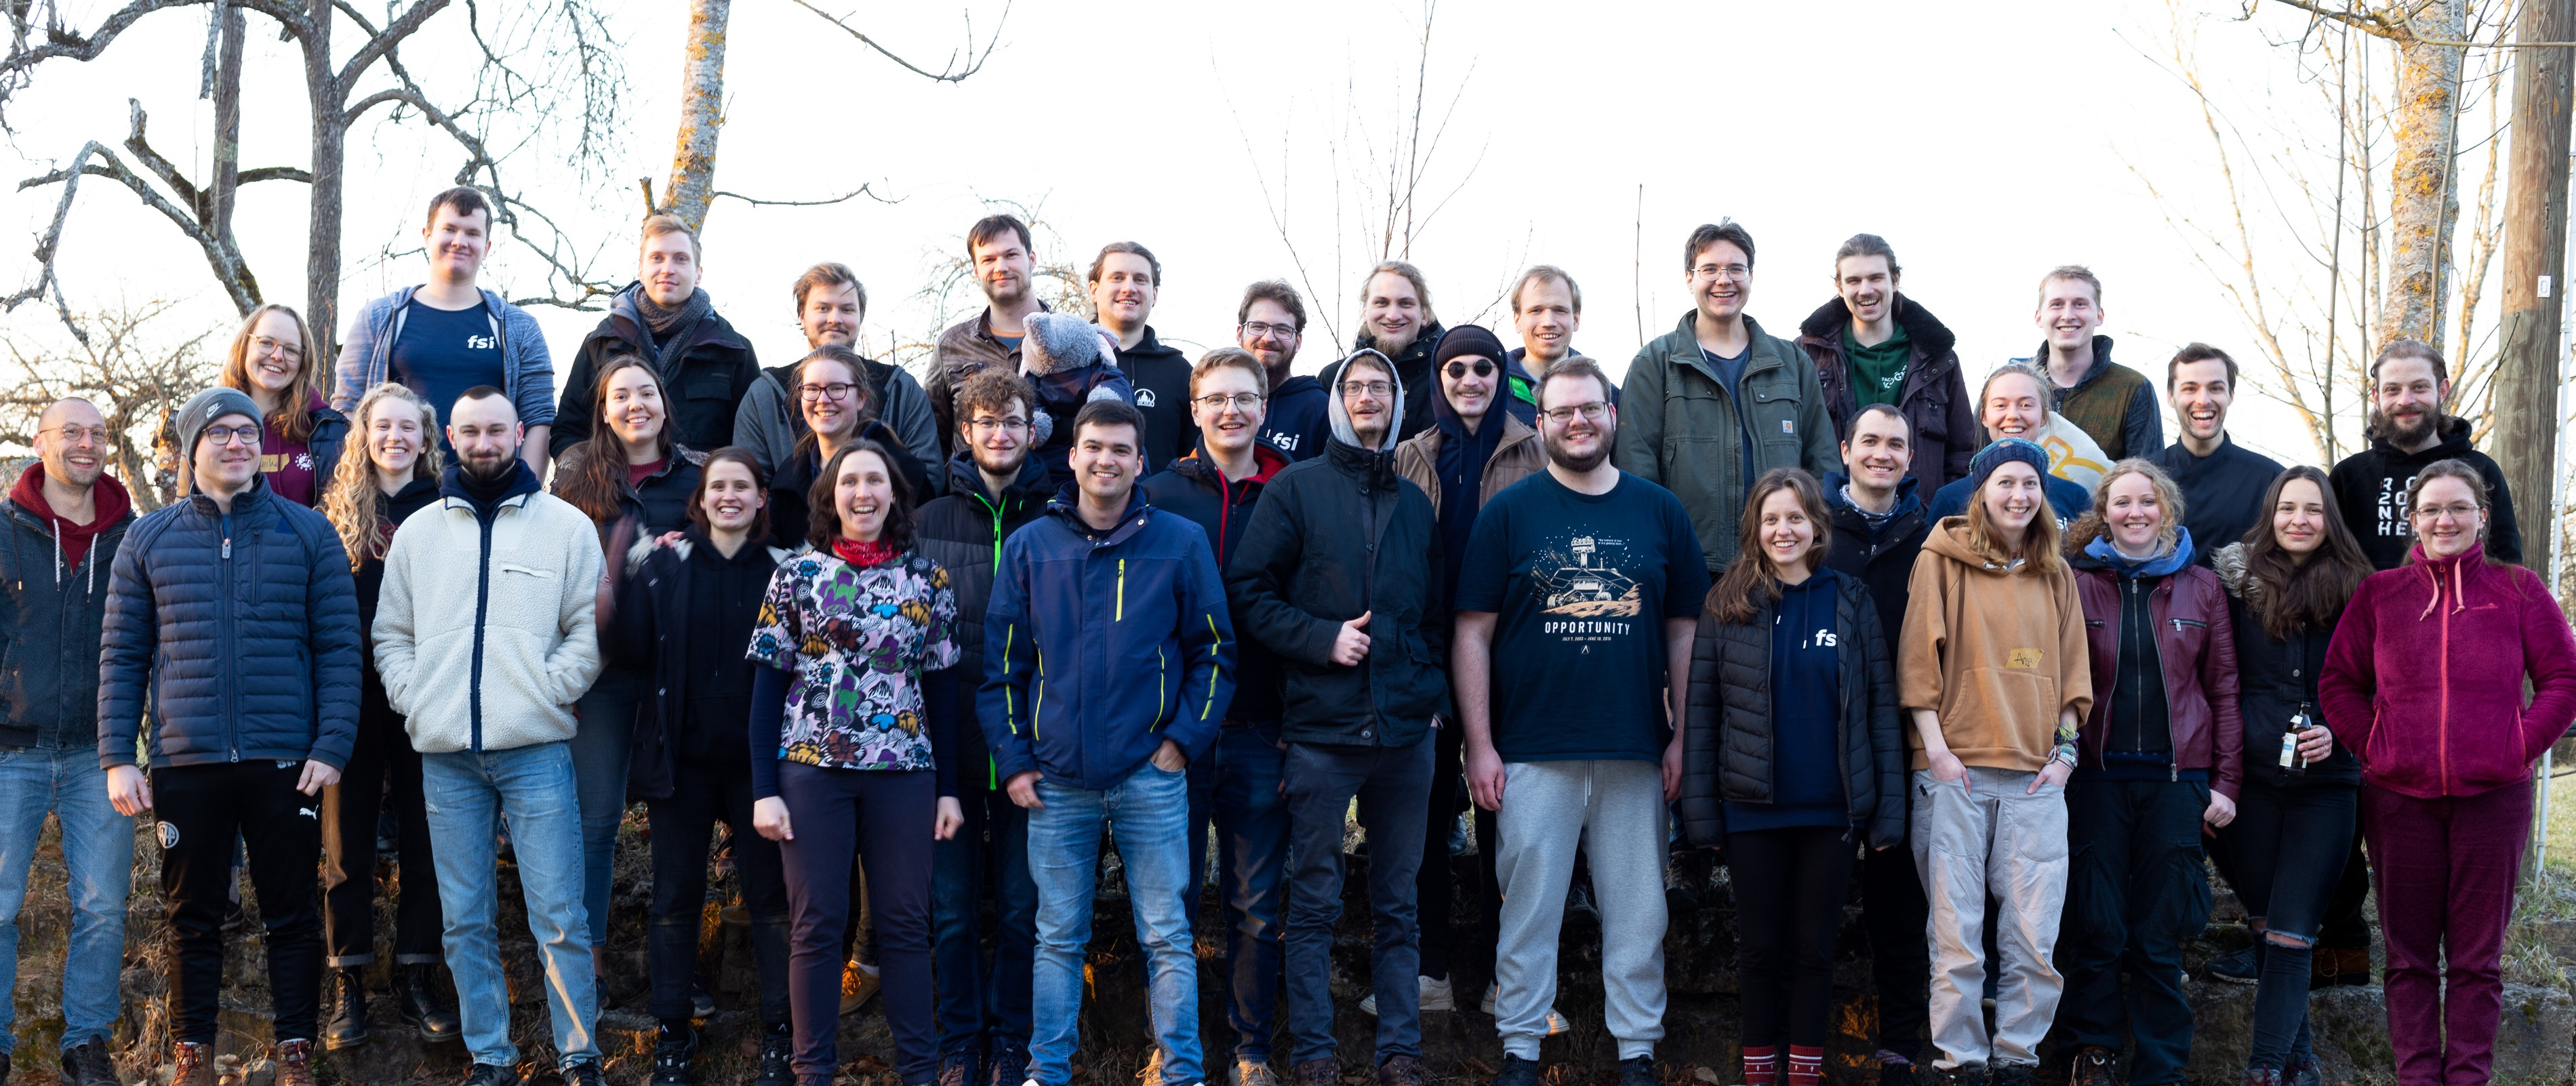
\includegraphics[height=\paperheight]{pictures/fsi_22.jpg} }

\begin{frame}
  \centering
  \vspace{.5cm}
  \includegraphics[height=.25\textheight]{pictures/fsi-denker.pdf} %
  \hspace{2em} %
  \includegraphics[height=.25\textheight]{pictures/fsk2.pdf}\\
  \vspace*{1cm}
  \begin{huge}
     \eventname
  \end{huge}

    \vspace{1.5cm}
    \semester
\end{frame}}

%= = = = = = = = = = = = = = = = = = = = = = = = = = = = = = = = = = = = = = = =
%   Table of Contents
%   =================
%
%   1. What did we do last year?
%   2. What upcoming events are there?
%      i. We need you for Studieninfotag!
%   ~~3. Workshop~~
%   4. Come and join us!
%= = = = = = = = = = = = = = = = = = = = = = = = = = = = = = = = = = = = = = = =


%-------------------------------------------------------------------------------
%   What did we do last year?
%-------------------------------------------------------------------------------

\section{What did we do last year?}
\begin{frame}{\insertsection}
    \begin{columns}
        \column{.5\textwidth}
        \centering
        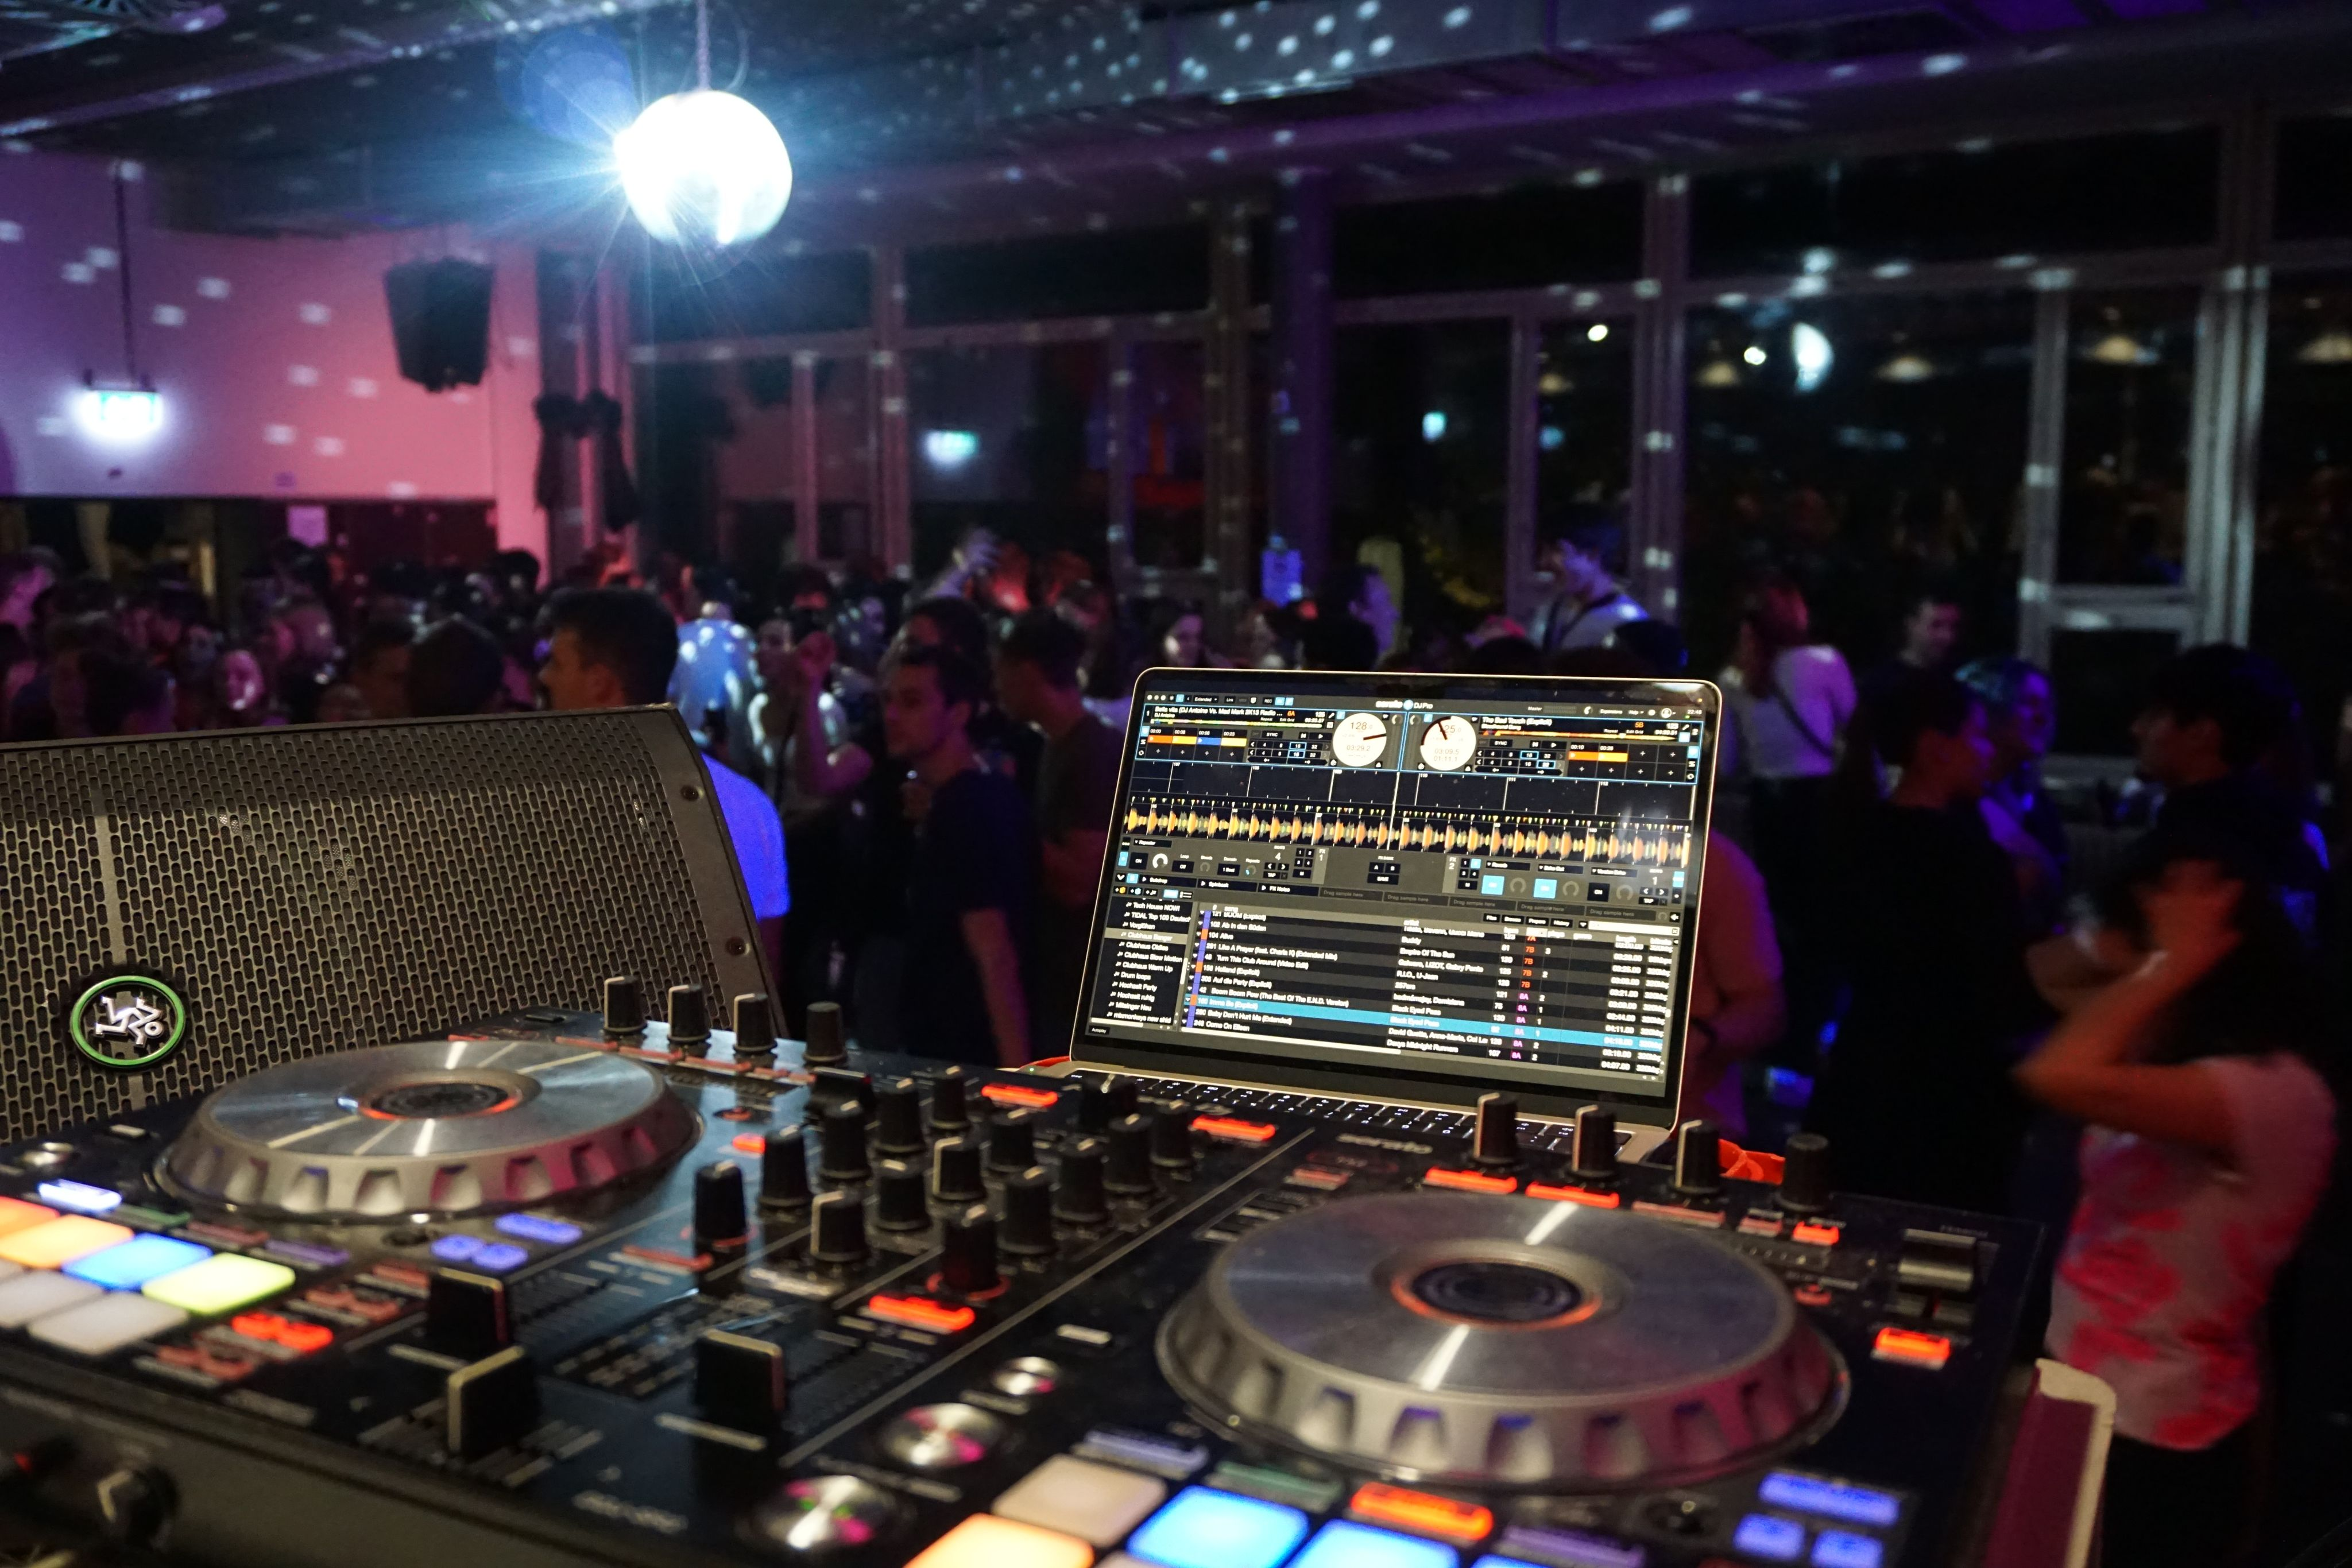
\includegraphics[width=.9\linewidth]{pictures/chfws23.jpg}
        
        \column{.5\textwidth}
        \begin{itemize}
            \item \textbf{Freshmen program} 
                  BBQs, \faDice Game Nights, \faFilm Movie Nights, \faBeer Pub Crawls, 
                  \faRoute City Rally, \faWalking Hikes, ...

            \item \textbf{\faMusic Clubhausfest}
            
            %\item \textbf{\faBeer Sommerfest} 

            \item \textbf{\faMugHot Christmas / Winter party}

            % \item \textbf{Workshops:} {\Large \faGit}, \LaTeX, \faPython Python
                  %{\footnotesize (Those in the summer term sadly were cancelled)}

            \item \textbf{Student Council Meetings} \\
                  $\approx 26$ meetings, $> 100$ topics
        \end{itemize}
        
    \end{columns}
\end{frame}

%-------------------------------------------------------------------------------
%   What upcoming events are there?
%-------------------------------------------------------------------------------

\section{What upcoming events are there?}

% TODO: Hintergrund anpassen (falls verfügbar)
% { \setbeamertemplate{background} {
%     \hspace{-1em} 
%     \transparent{0.1}
%     
\includegraphics[width=\paperwidth]{pictures/pink.png} }

\begin{frame}{\insertsection}
    \begin{columns}
        \column{.5\textwidth}
        \centering
        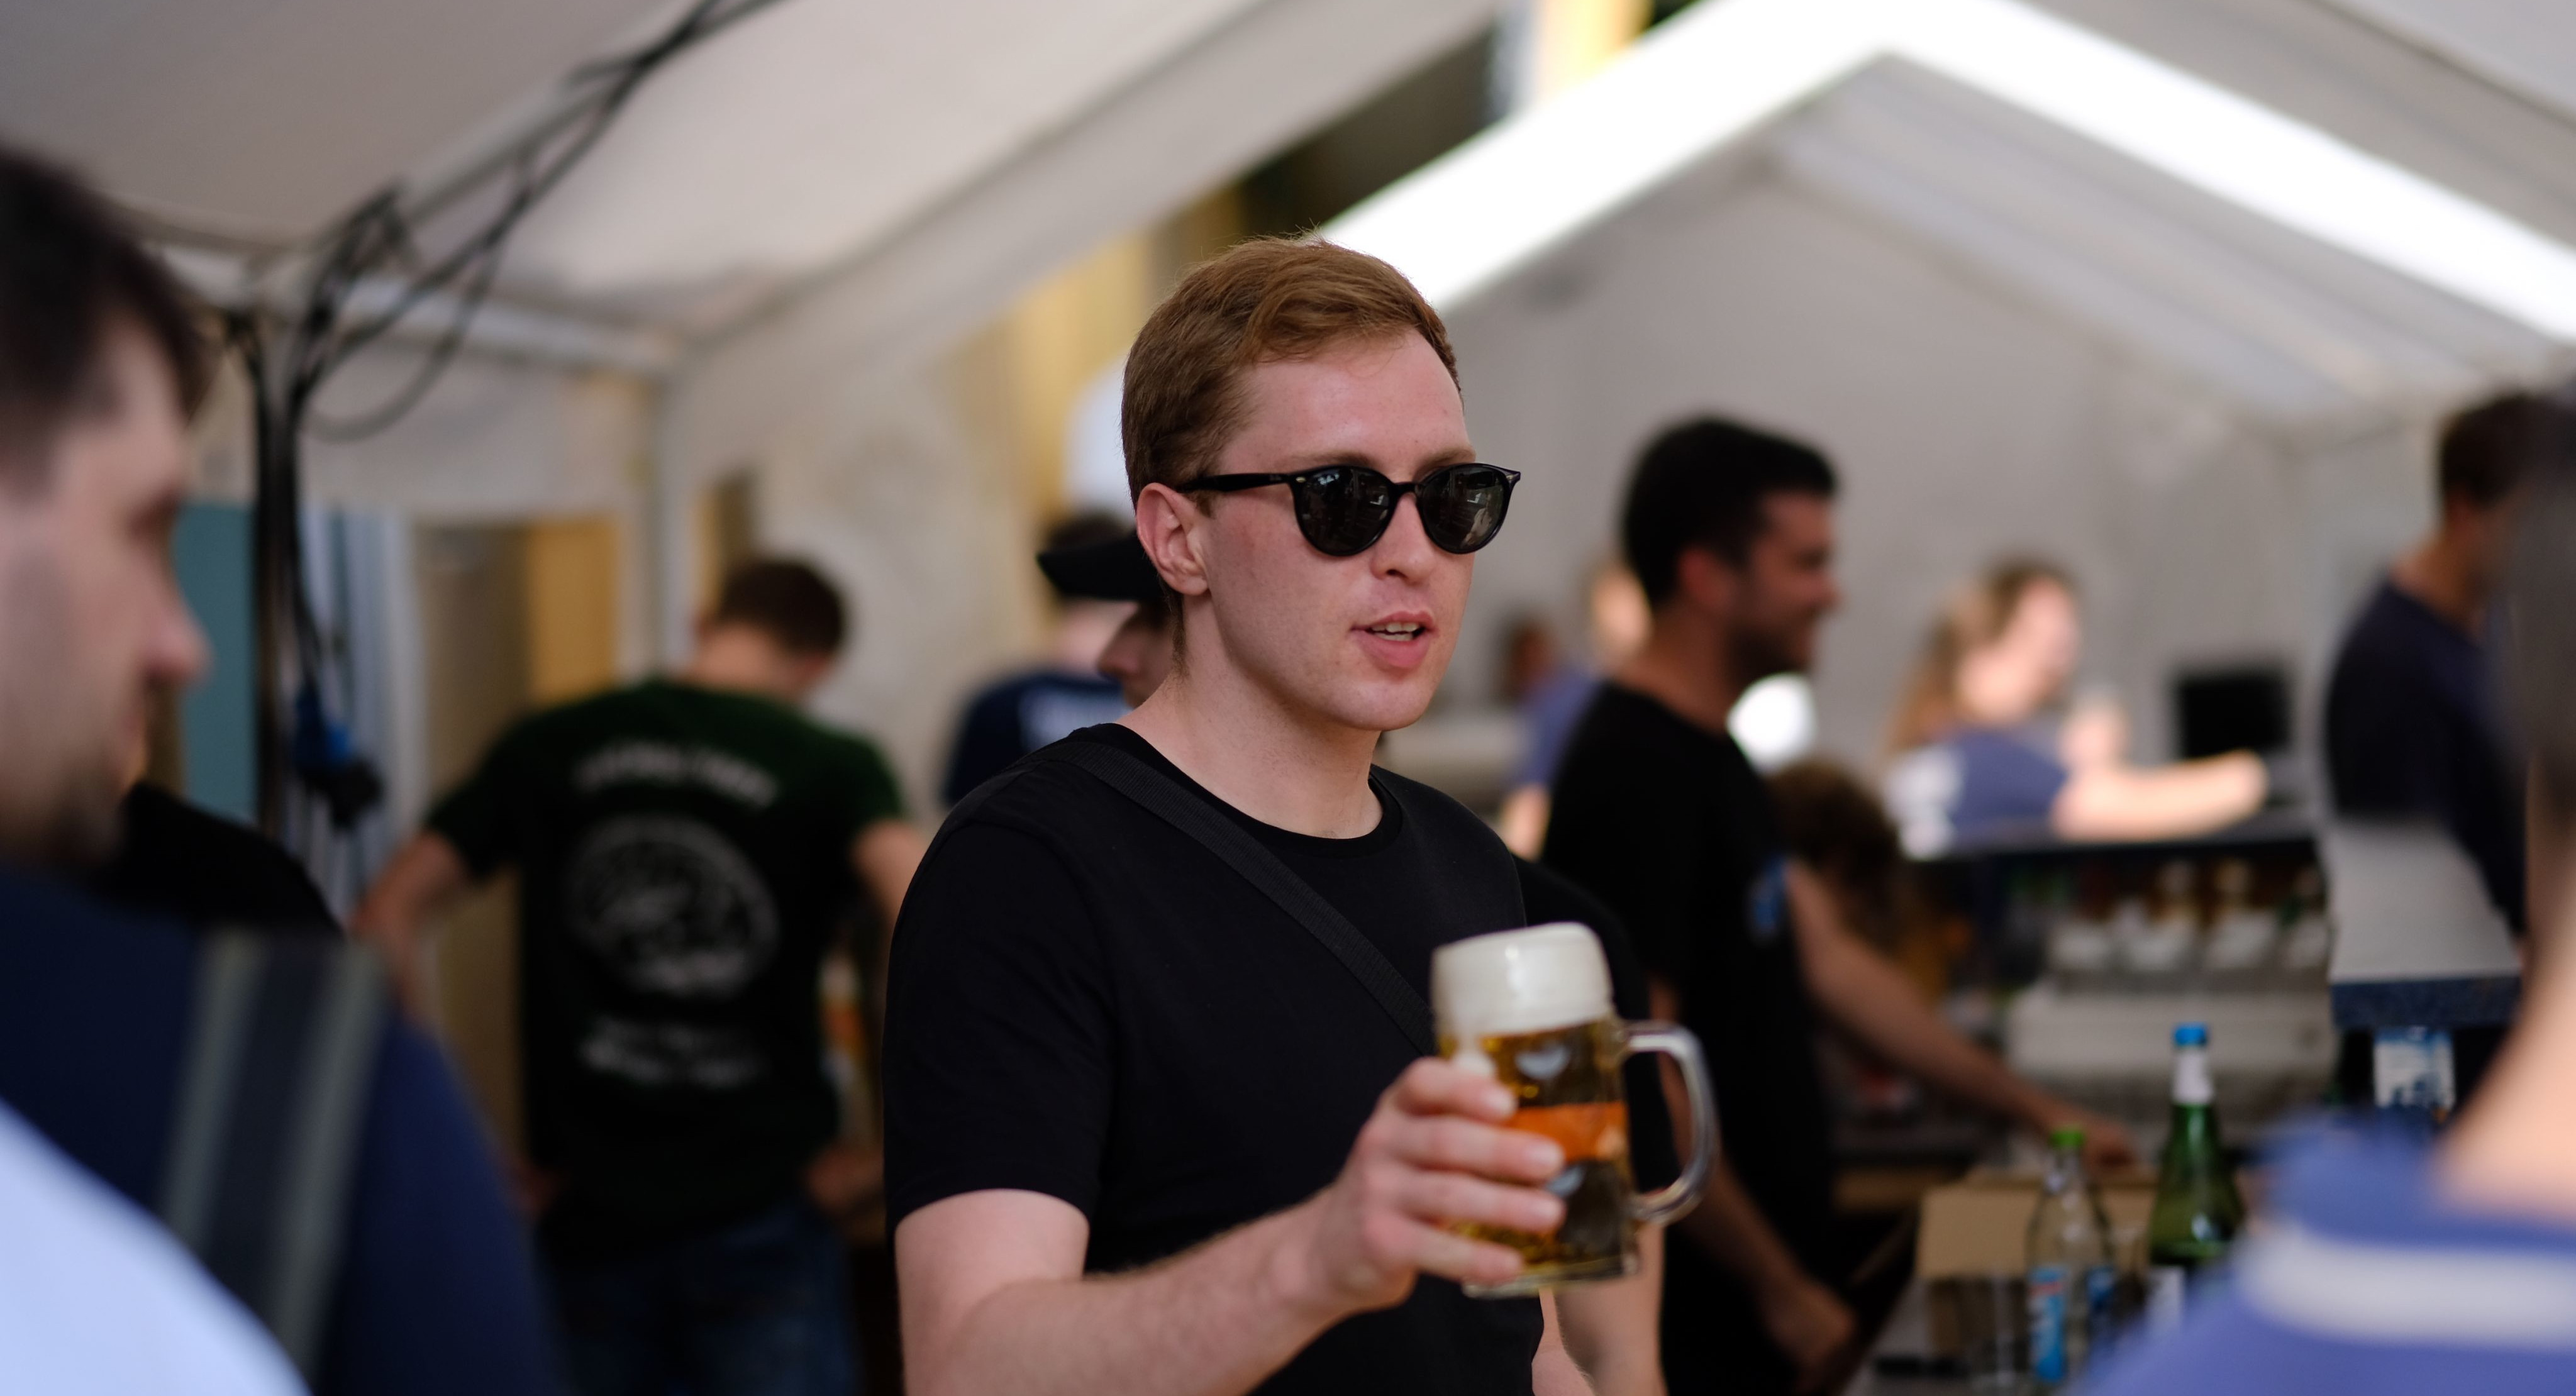
\includegraphics[width=.9\linewidth]{pictures/sommerfest3_crop.jpg}
        \begin{minipage}{.9\linewidth}
            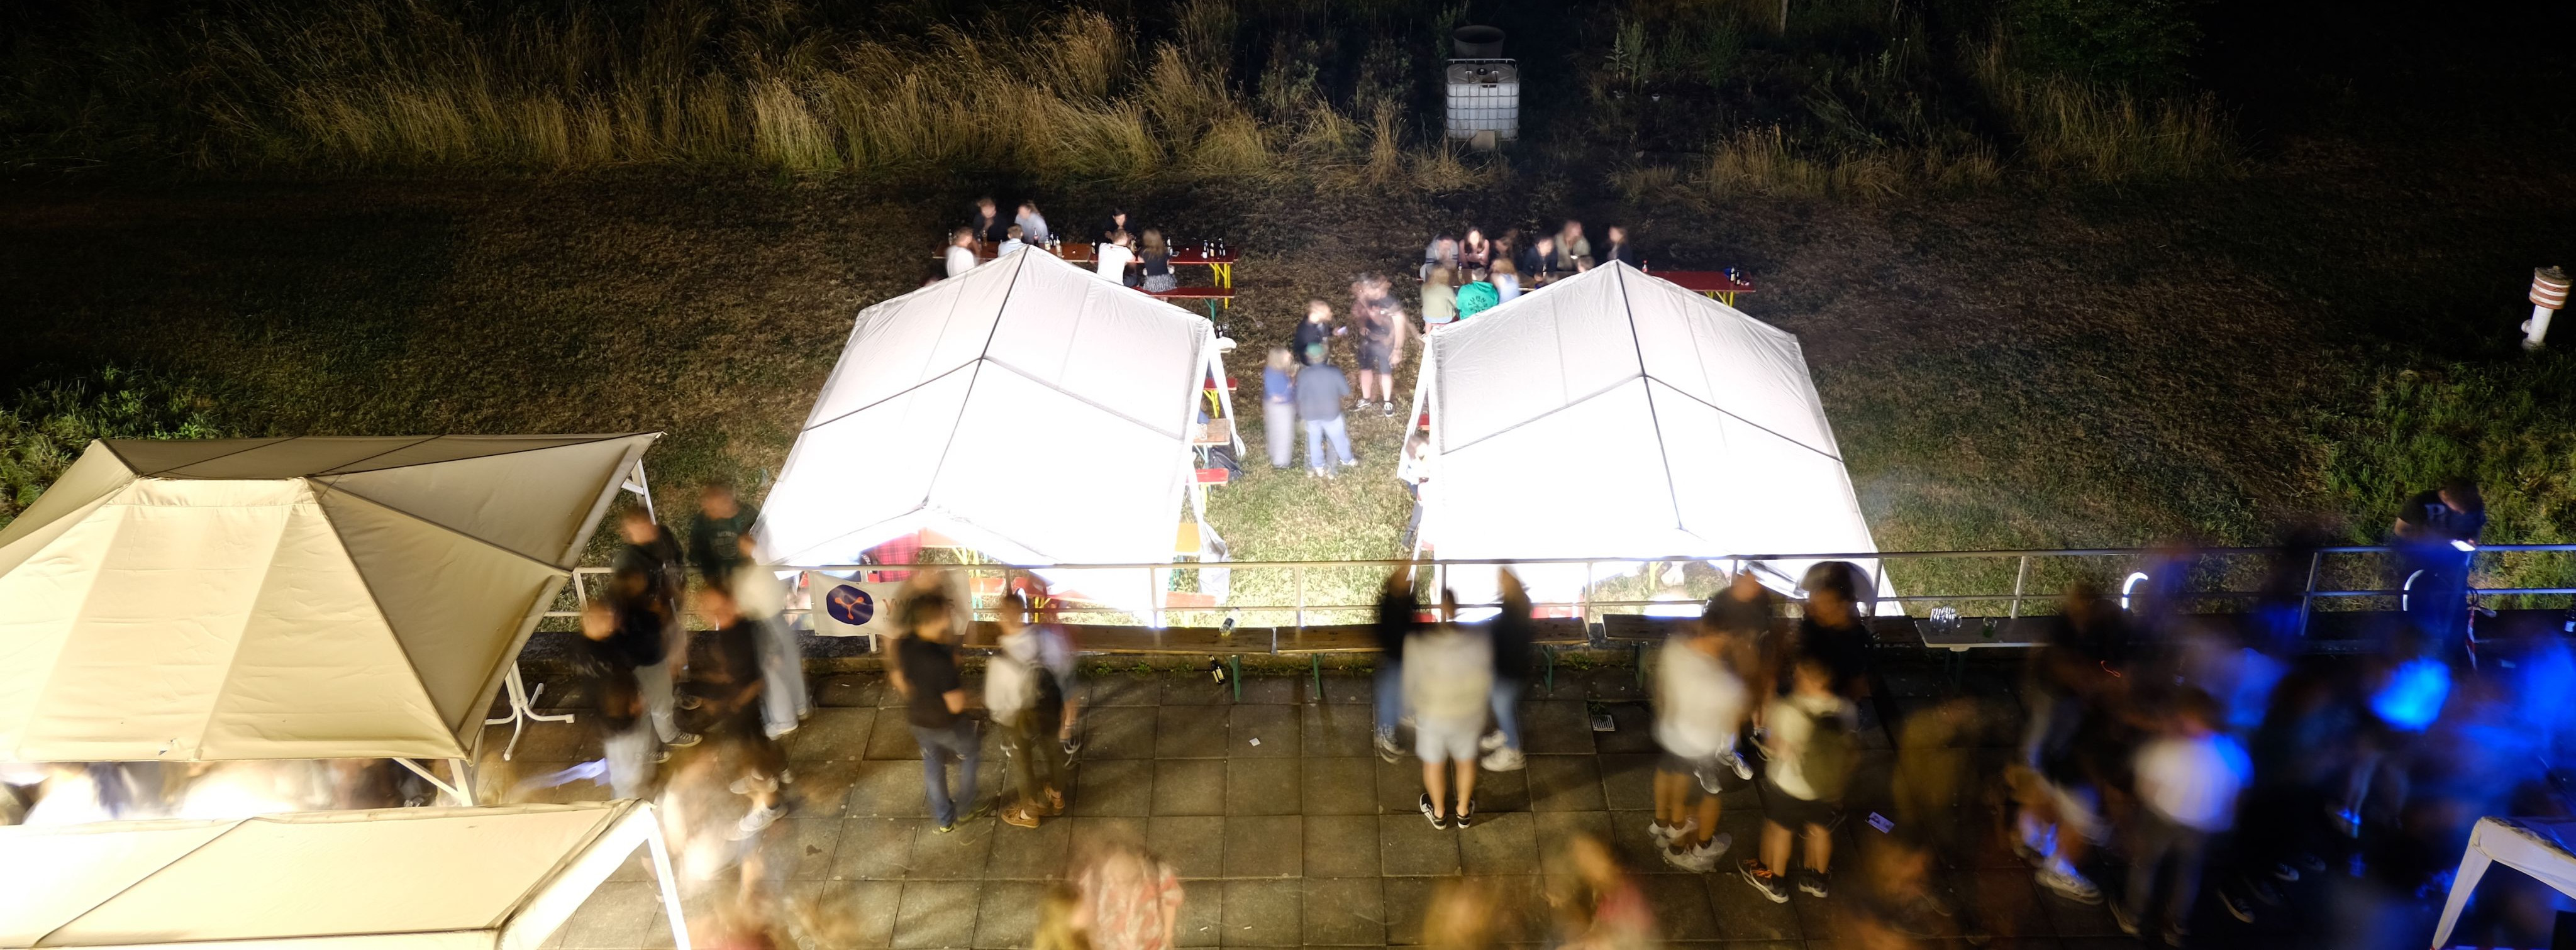
\includegraphics[height=.2575\linewidth]{pictures/sommerfest_crop.jpg}
            
\includegraphics[height=.2575\linewidth]{pictures/skipper.png}
        \end{minipage}
        
        \column{.5\textwidth}
        \begin{itemize}
            \item \textbf{\faMusic Clubhausfest (\dateCHF)}\\
                  With the Fachschaften \emph{Cognitive Sciences}, \emph{Informatics}, \emph{Psychology} and \emph{Political Science} \\
                  or sKIPPer for short

            \item \textbf{\faBeer Sommerfest (\dateSommerfest)} 
            % \item \textbf{\faMugHot Christmas / Winter party}

            \item \textbf{Workshops} 
                  {\footnotesize What topics would you like? 
                  Do you want to give a lightning talk?}
            
        \end{itemize}
    \end{columns}
\end{frame}


\subsection{Upcoming}
\begin{frame}{\insertsubsection}
    \centering
    
\includegraphics[width=.9\linewidth]{pictures/xrlab.png}
    \vspace{1em}

    \begin{tabular}{cl}
        \color{fskgreen}\faMicroscope  & Experiment with XR Technology \\
        \color{fskgreen}\faVrCardboard & VR Goggles with Eye-Tracking \\
        \color{fskgreen}\faServer      & High-End Computer \\
        \color{fskgreen}\faHammer      & Currently under construction \\
    \end{tabular}
 
    \vspace{1em}
    \textbf{we will keep you informed!}
\end{frame}

% % Nur Wintersemester
% \subsection{Studieninfotag (22.11.)}
% \begin{frame}{\insertsubsection}

%   \centering
%   
\includegraphics[height=.6\textheight]{pictures/studieninfotag1.jpg}
%   
\includegraphics[height=.6\textheight]{pictures/studieninfotag2.jpg}
  
%   \vspace{1em}

%   Are you interested to represent your subject of studies? \\
%   \emph{Hit us up at} \faEnvelope \texttt{\url{fsi@fsi.uni-tuebingen.de}}

% \end{frame}


% %-------------------------------------------------------------------------------
% %   Solder, Print and Repair Shop
% %-------------------------------------------------------------------------------
% 
% \section{Solder, Print and Repair Shop}
% 
% { \setbeamertemplate{background} {
%     \hspace{-10em} 
%     \transparent{0.2}
%     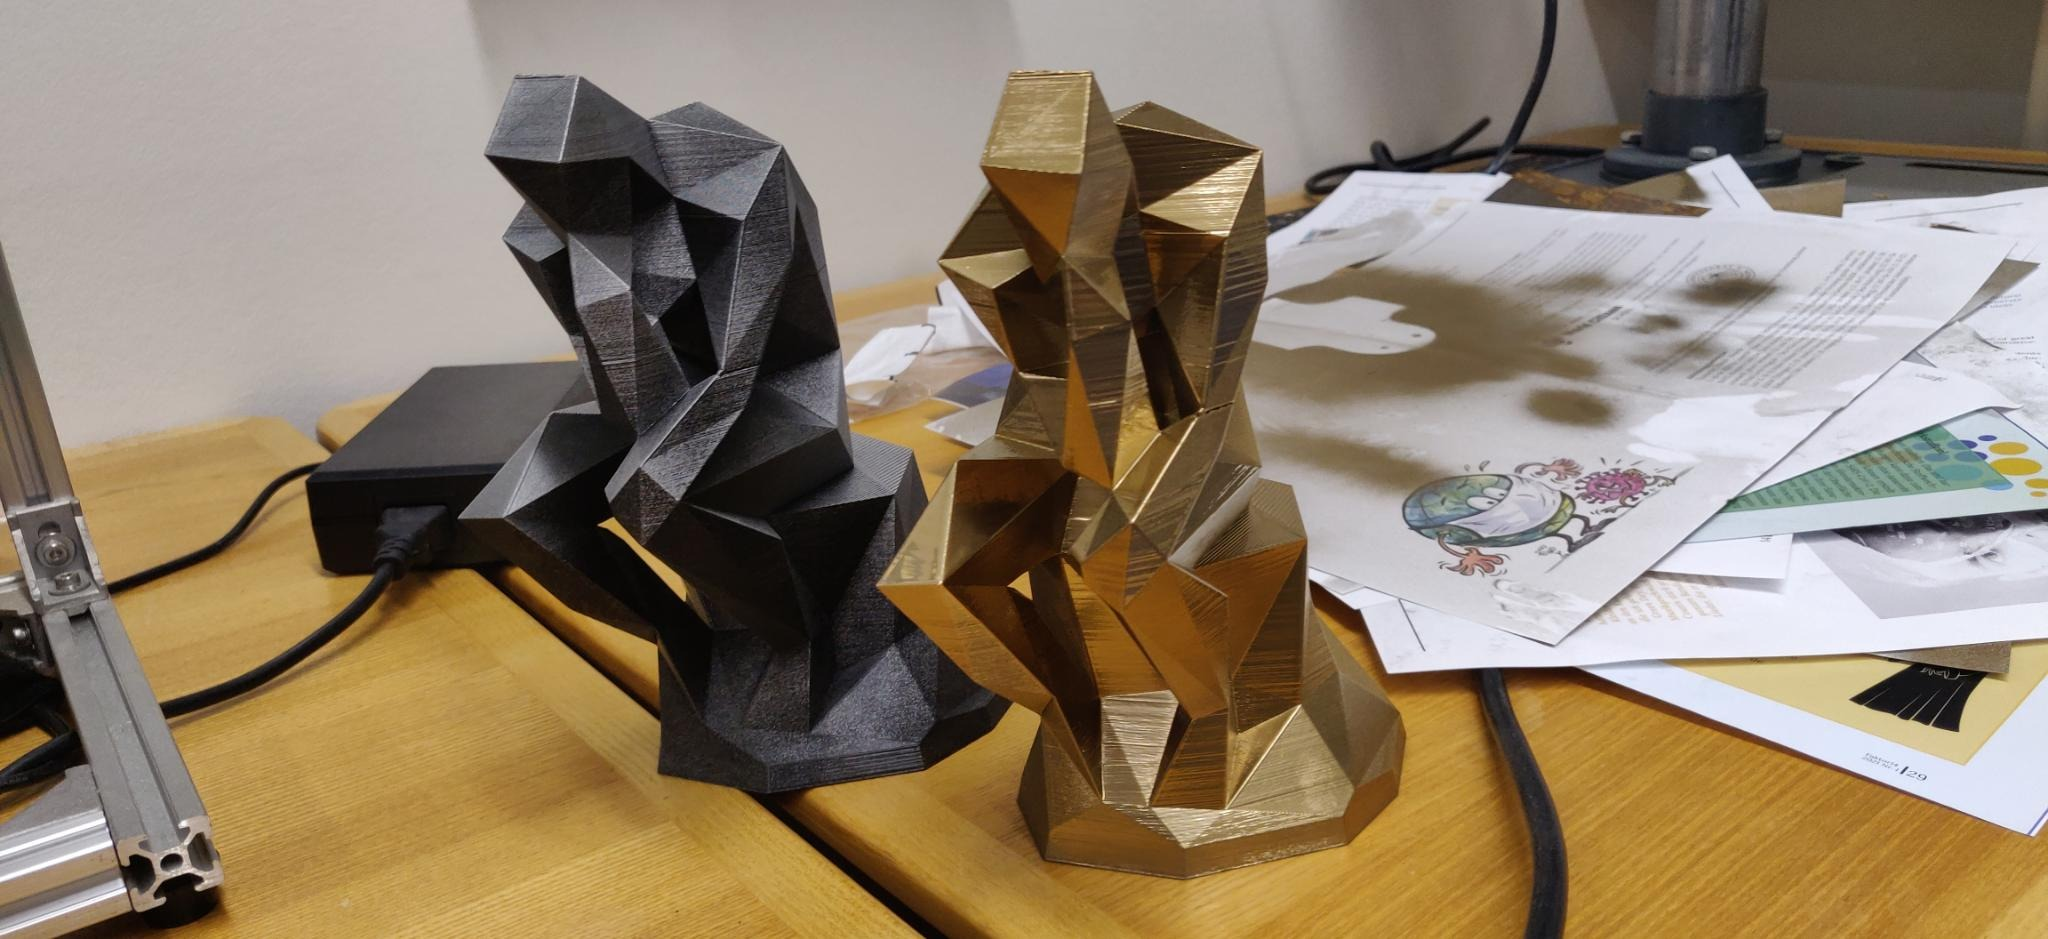
\includegraphics[height=\paperheight]{pictures/werkstatt.jpeg} }
% 
% \begin{frame}{\insertsection}
%     \begin{columns}
%         \column{.7\textwidth}
%         \centering
%         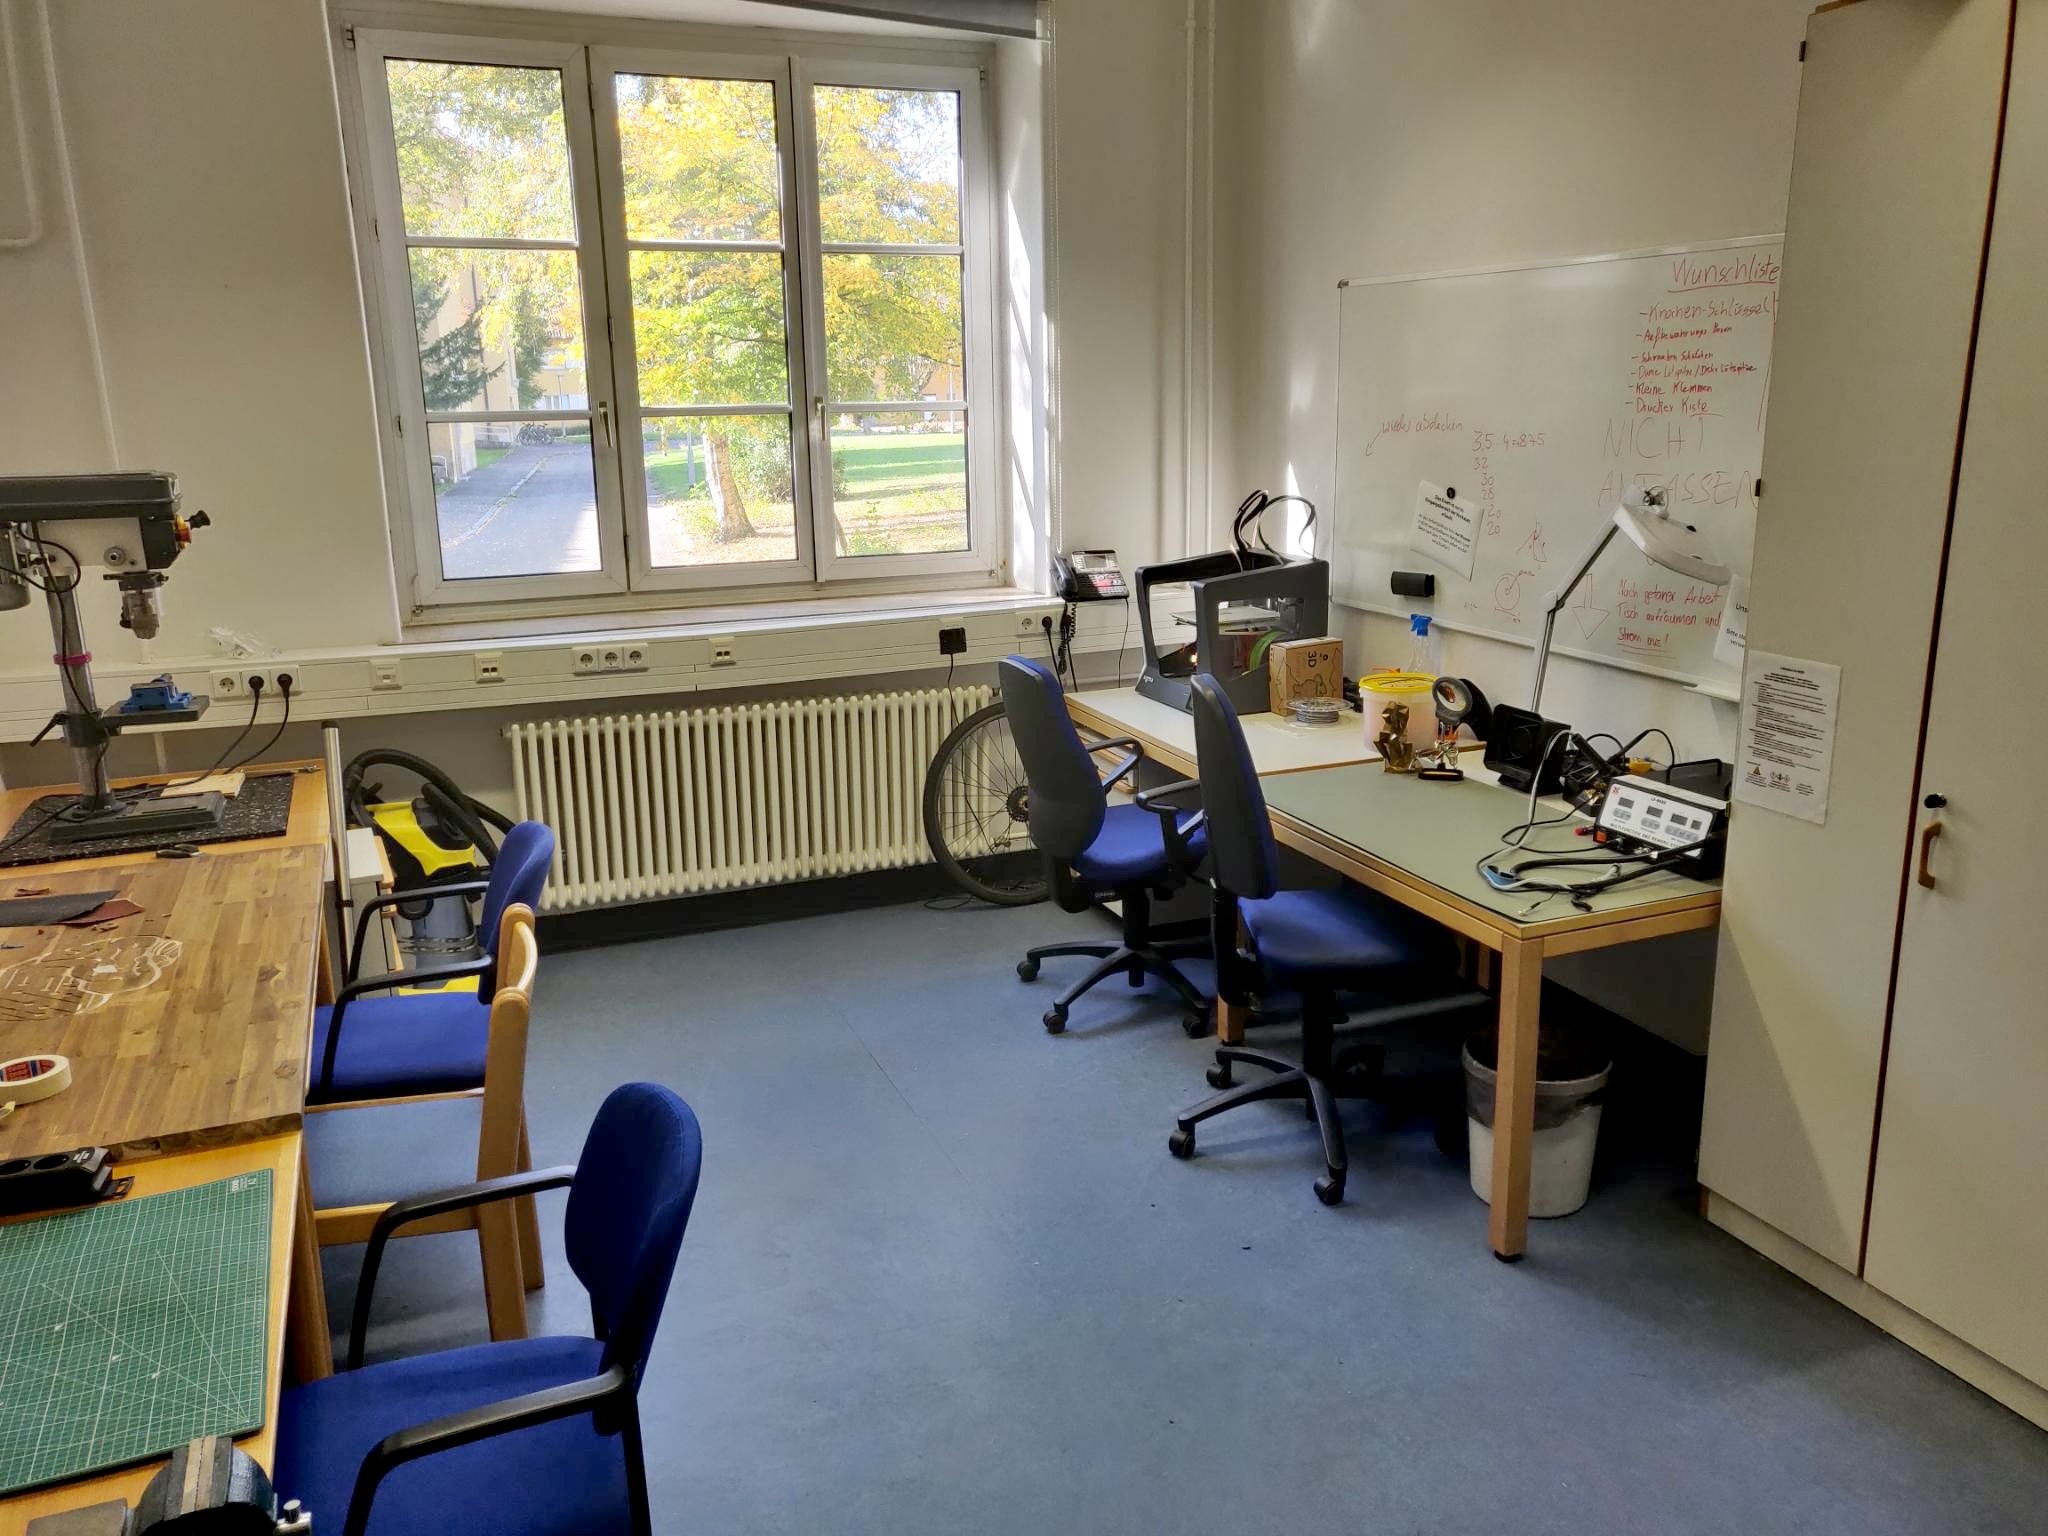
\includegraphics[height=.6\textheight]{pictures/Werkstatt.jpeg}
%         \begin{itemize}
%             \large
%              \item \textbf{Meet and collaborate} 
%              \item \textbf{New Skills}
%              \item \textbf{Tools:} Common tools, Drill Press, Soldering Station, 3D printer 
%         \end{itemize}
%          
%         \column{.3\textwidth}
%         \centering
%         {\large \color{darkgray} \textbf{Infos / Booking}}\\[1em]
%         \scalebox{1.5}{\fancyqr[color=darkgray]{\linkAnmeldung}}
%         \\[1em]
%         {\footnotesize \url{\linkAnmeldung}}
%     \end{columns}
% \end{frame} }

%-------------------------------------------------------------------------------
%   Other Things We Do
%-------------------------------------------------------------------------------
\section{ Other Things We Do } % TODO besseren section title finden

{ \setbeamertemplate{background} {
    \hspace{-10em} 
    \transparent{0.2}
    }

\begin{frame}{\insertsection}
    \begin{columns}
        \column{0.7\textwidth}
        \centering
        \begin{itemize}
            \large
            \item \textbf{University committees}: \\
            \begin{itemize}
                \item Examination Board {\footnotesize (Prüfungsausschuss)} \\
                \item Study Commmission {\footnotesize (Studienkommission)}\\
                \item Appointment Committees {\footnotesize (Berufungskommissionen)}
                % \item \(\dots\)
            \end{itemize}
            % \item \textbf{Study information days} 
            \item \textbf{Mailing lists:} \\
            info-studium, info-talk, info-jobs,...\\
            \item \textbf{Infrastructure}
        \end{itemize}
         \column{.3\textwidth}
         \centering
          {\large \color{darkgray} \textbf{tool collection}}\\[1em]
         \scalebox{1.5}{\fancyqr[color=darkgray]{\linkTools}}
         \\[1em]
         {\footnotesize \url{\linkTools}}
    \end{columns}
\end{frame} }


%-------------------------------------------------------------------------------
%   Appointment committeess
%-------------------------------------------------------------------------------
\section{ Appointment committees (Berufungskommissionen) }

{ \setbeamertemplate{background} {
    \hspace{-10em} 
    \transparent{0.2}
    }

\begin{frame}{\insertsection}
    \begin{columns}
    \centering
    \column{.30\textwidth}
        \centering
        
\includegraphics[width=\linewidth]{pictures/uncle_sam_bk.jpg}\\
    \column{.60\textwidth}
        \Large {You want to help choosing the next professor? \\ \textbf{Join an appointment committee!}}
    \end{columns}
\end{frame} }


%-------------------------------------------------------------------------------
%   Come and join us!
%-------------------------------------------------------------------------------

\section{Come and join us!}
\begin{frame}{\insertsection}
    \centering 
    \begin{columns}[b]
    \column{.5\textwidth}
    \Large
    {\Huge\color{fsiblue} \faClock[regular]}   \timeSitzung 

    \vspace{4em}
    {\Huge\color{fsiblue} \faMapMarker*} \locFSI\\[.5em]

    \vspace{.2em}
    \small
    \faInstagram \href{https://www.instagram.com/fsi\_tuebingen/}{%
                      \texttt{@fsi\_tuebingen}} \\
    \faMastodon \href{https://toot.kif.rocks/@fsi\_tue}{%
                      \texttt{@fsi\_tue@toot.kif.rocks}} \\
    \faLink \url{https://www.fsi.uni-tuebingen.de} \\
    \faEnvelope \url{fsi@fsi.uni-tuebingen.de} \\

    \column{.5\textwidth}
    \centering
    
\includegraphics[width=\textwidth]{pictures/you-want-to.jpg}
    
    \vspace{1.2em}

    \flushleft
    \Large
    {\Huge\color{fskgreen} \faMapMarker*} \locFSK\\[.5em]

    \vspace{.8em}
    \small
    \faInstagram \href{https://www.instagram.com/fsk.tuebingen/}{%
                        \texttt{@fsk.tuebingen}} \\
    \faLink \url{https://www.fs-kogni.uni-tuebingen.de} \\
    \faEnvelope \url{kogni-fachschaft@fsi.uni-tuebingen.de} \\

    \end{columns}
\end{frame}

% - - - Animation -------------------------------------------------------------
\begin{frame}{\insertsection}
    \centering 
    \begin{columns}[b]
    \column{.5\textwidth}
    \color{fsiblue}

    \centering
    % \qrcode[height=.6\textwidth]{\linkFSI}
    % \scalebox{2}{\fancyqr[color=fsiblue]{\linkFSI}}
    % \flushleft
    \scalebox{2}{\fancyqr[
        image=\bfseries\itshape\hspace{-.5em} fsi, 
        image x padding=1, color=fsiblue]{\linkFSI}}
    \flushleft

    \vspace{1em}
    \small
    \faInstagram \href{https://www.instagram.com/fsi\_tuebingen/}{%
                      \texttt{@fsi\_tuebingen}} \\
    \faMastodon \href{https://toot.kif.rocks/@fsi\_tue}{%
                      \texttt{@fsi\_tue@toot.kif.rocks}} \\
    \faLink \url{\linkFSI} \\
    \faEnvelope \url{fsi@fsi.uni-tuebingen.de} \\

    \column{.5\textwidth}
    \color{fskgreen}

    \centering
    % \qrcode[height=.6\textwidth]{\linkFSK}
    \scalebox{2}{\fancyqr[
        image=\bfseries\itshape\hspace{-.5em} fsk, 
        image x padding=0, color=fskgreen]{\linkFSK}}
    \flushleft
    
    \vspace{1.7em}
    \small
    \faInstagram \href{https://www.instagram.com/fsk.tuebingen/}{%
                      \texttt{@fsk.tuebingen}} \\
    \faLink \url{\linkFSK} \\
    \faEnvelope \url{kogni-fachschaft@fsi.uni-tuebingen.de} \\

    \end{columns}
\end{frame}

%-------------------------------------------------------------------------------
\end{document}

